\subsection{Analytical Comparisons}

This section will analyze and compare the simulated results with analytical solutions. I will begin by discussing the consumption rate and comparing the optimal consumption determined analytically with the data obtained from the policy network after training. I will then evaluate the abatement rate, examine how well the simulation aligns with closed-form solutions, and briefly touch on the SCC.

\subsubsection{The Consumption Rate}

As shown in equation (\ref{eq:analytical_x_t}), the analytical consumption rate suggests that the optimal consumption rate remains constant over time, independent of the states visited. Figure (\ref{fig:consumption rate, est vs. analytical}) illustrates the analytical consumption rate alongside the estimated rates derived from the best-performing policy network weights, following the second training cycle for the DICE 2016 and 2023 versions of ACE.

\begin{figure}[ht]
  \centering
  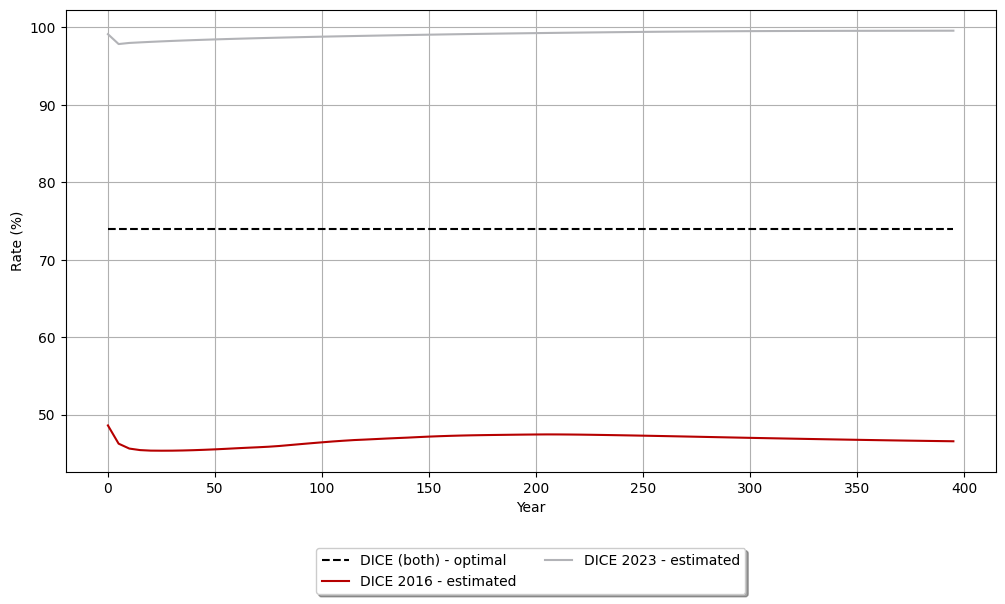
\includegraphics[width=1.0\textwidth]{images/ch6/estimated controls/x_1, estimated vs. optimal.png}
  \caption{Consumption rate, estimated versus analytical}
  \label{fig:consumption rate, est vs. analytical}
\end{figure}

The estimated consumption rates significantly deviate from the analytical consumption rate. Specifically, estimates from the 2016 version consistently remain below 50\% throughout the simulation, whereas estimates from the 2023 version approach a consumption rate close to 100\%. These deviations reflect the errors in the Lagrange condition on consumption and the Bellman equation, which recorded the highest errors in the final simulation runs. Notably, despite these discrepancies, the consumption rates from both estimates maintain stability, which is consistent with the analytical solution.

Compared to the analytical solution, the 2016 model’s lower consumption rate suggests an economic scenario where too little is consumed and too much is invested. This path implies that an economic agent following this strategy would benefit from increasing consumption today rather than investing today. Conversely, the 2023 model presents a scenario where consuming less today would give a more optimal path. This agent would benefit from investing more, leading to increased future production from which it could consume and get more utility. In this way, both simulated consumption paths are bad at considering the future, as evidenced by the significant errors in the Bellman equation.

\subsubsection{The Abatement Rate}
Figure (\ref{fig:social_cost_of_carbon_plot}) illustrates the calculated SCC values for the DICE 2016 and DICE 2023 versions of ACE. Recall that the SCC (eq. \ref{eq:analytical_scc}) depends on the simulated outputs and temperatures though the damage function and the exogenous backstop price exogenously defined in the respective DICE versions\footnote{See appendix (\ref{apdx:simulation-initializations}) for the definition and initialization of the backstop price.}.

We observe that the SCC for the 2016 version is higher than that of the 2023 version. This discrepancy can largely be attributed to the nearly 100\% consumption rate observed in the 2023 version, which significantly restricts output growth. In the DICE model, business-as-usual emissions are directly tied to output. Consequently, lower output leads to lower CO$_2$ emissions, which in turn results in lesser atmospheric temperature increases and, subsequently, lower associated damages. This contributes to a lower SCC for the 2023 version until production escalates, aided by a significantly higher path of total factor productivity compared to the 2016 version over the simulated path.

\begin{figure}[ht]
  \centering
  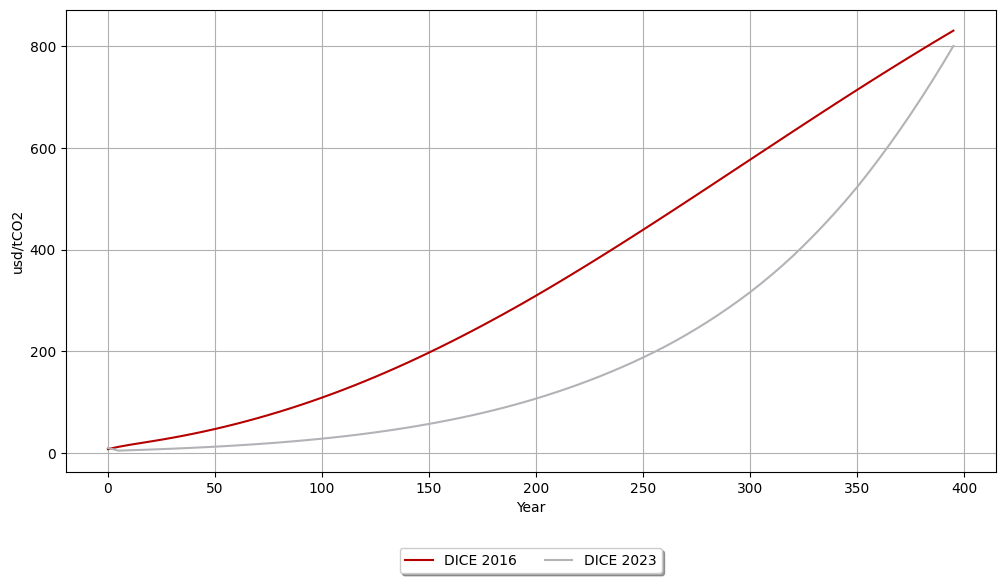
\includegraphics[width=1.0\textwidth]{images/ch6/SCC.png}
  \caption{SCC in USD/tCO$_2$}
  \label{fig:social_cost_of_carbon_plot}
\end{figure}

With this analysis, we can determine the optimal abatement rates for each model and compare these to the ratio of the neural network emissions estimates to the business-as-usual emissions. The outcomes are presented in Figure (\ref{fig:abatement rate, est vs. analytical}).

\begin{figure}[ht]
  \centering
  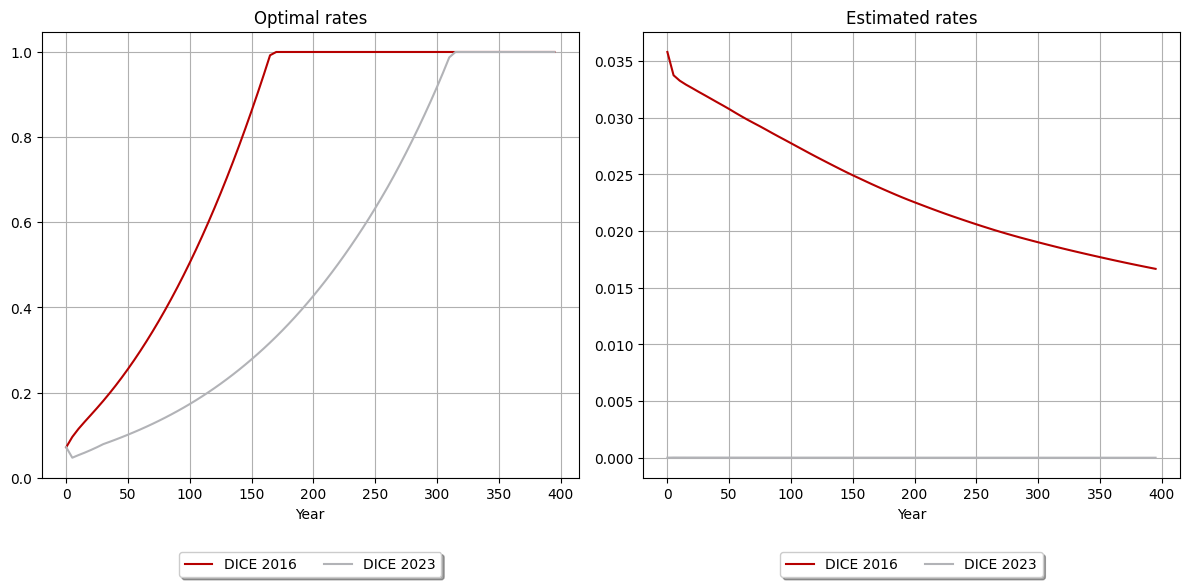
\includegraphics[width=1.0\textwidth]{images/ch6/estimated controls/mu_t, estimated vs. optimal.png}
  \caption{Abatement rate, estimated versus analytical}
  \label{fig:abatement rate, est vs. analytical}
\end{figure}

As we observed with the SCCs, the optimal abatement rates derived from the analytical solutions for the 2023 version lag behind the 2016 version. This follows the same rationale discussed previously, where economic dynamics affecting the SCC similarly influence the abatement rates. 

The abatement rates estimated by the policy network show significant deviations from the analytical predictions; notably, the 2023 version's estimated abatement rate is nearly zero, and the rate for the 2016 version declines over time, contradicting expectations of an increase. These discrepancies reflect the errors in the Lagrange condition on emissions \(\ell_4\) and the Bellman equation, which are the objective functions with some of the largest errors. 

The estimated abatement rates are suboptimal, as they allow too much CO$_2$ to accumulate in the atmosphere, leading to higher temperatures and substantial damages to output. This results in lower future consumption since consumption is directly linked to output, thus also reducing utility. Therefore, the agent would benefit from incurring some abatement costs to reduce CO$_2$ emissions, which would subsequently minimize damages to output and preserve higher levels of future consumption and utility.